% Baccalauréat malgache, série D, 2007 : énoncé.
\TCDBacAttribution{D}{2007}
\providecommand{\Courbe}{(\mathscr{C})}
\providecommand{\D}{(\mathscr{D})}
\providecommand{\Plan}{(\mathscr{P})}
\providecommand{\Ouv}{(O ; \vec{u} , \vec{v})}
%\providecommand{\Oij}{(O ; \vec{\imath} , \vec{\jmath})}
\providecommand{\cm}{~\mathrm{cm}}
\providecommand{\dx}{~\mathrm{d}x}
\providecommand{\Arg}[1]{\mathrm{Arg}\left( #1 \right)}
\providecommand{\Angl}[2]{\left( \overrightarrow{#1} ; \overrightarrow{#2} \right)}

\noindent \underline{\textsc{Exercice I}} (5 points) \newline
      Soit le polyn\^ome $P$ \`a variable complexe $z$ d\'efini par : 
      $P(z) = z^3 + (1+i) z^2 + (4-i) z - 6i + 12$.
      \begin{enumerate}
            \item \begin{enumerate}
                        \item Calculer $P(-3i)$.
	                        \item Montrer que l'\'equation $P(z) = 0$ admet une solution r\'eelle $\alpha$ que l'on d\'eterminera.
                        \item D\'eterminer le nombre complexe $\beta$ tel que $P(z)$ peut s'\'ecrire sous la forme :
                              $P(z) = (z+3i) (z+2) (z+\beta)$.
                        \item R\'esoudre dans $\mathbb{C}$ l'\'equation $P(z) = 0$.
                  \end{enumerate}
            \item Dans le plan complexe $\Plan$ muni d'un rep\`ere orthonorm\'e $\Ouv$, on consid\`ere les points 
                  $A$, $B$, $C$ d'affixes respectives $z_A = -3i$ ; $z_B = -2$ et $z_C = 1 + 2i$.
                  D\'eterminer la mesure de l'angle $\Angl{BA}{BC}$ et $\left| \frac{z_C - z_B}{z_A - Z_B} \right|$
                  puis en d\'eduire la nature du triangle $ABC$.
            \item Soit $r$ la rotation de centre $B$ et d'angle $\frac{\pi}{2}$.
                  Ecrire l'expression complexe de la rotation $r$.
            \item On consid\`ere la transformation $S$ du plan $\Plan$ dans $\Plan$ qui \`a tout point $M$
                  d'affixe $z$ associe le point $M'$ d'affixe $z'$ tel que $S\ :\ z' = 2iz - 2 + 4i$.
                  \begin{enumerate}
                        \item Donner la nature et les \'el\'ements caract\'eristiques de $S$.
                        \item Donner la nature et les éléments caractéristiques de la transformation $h$ telle que
                              $r \circ h = S$.
                  \end{enumerate}
      \end{enumerate}
%%%%%%%%%%%%%%%%%%%%%%%%%%%%%%%%%%%%%%%%%%%%%%%%%%%%%%%%%%%%%%%%%%%%%%%%%%%%%%%%%%%%%%%%%%%%%%%
%%%%%%%%%%%%%%%%%%%                   %%%%%%%%%%%%%%%%%%%                   %%%%%%%%%%%%%%%%%%%
%%%%%%%%%%%%%%%%%%%%%%%%%%%%%%%%%%%%%%%%%%%%%%%%%%%%%%%%%%%%%%%%%%%%%%%%%%%%%%%%%%%%%%%%%%%%%%%
\noindent \underline{\textsc{Exercice II}} (5 points) \newline
      Un sac contient six jetons, portant les lettres A, B, C et D dont la répartition suivant les
      couleurs est donnée par le tableau ci-dessous :
      \par\smallskip\noindent
      \adjustbox{max width=\linewidth,center}{%
      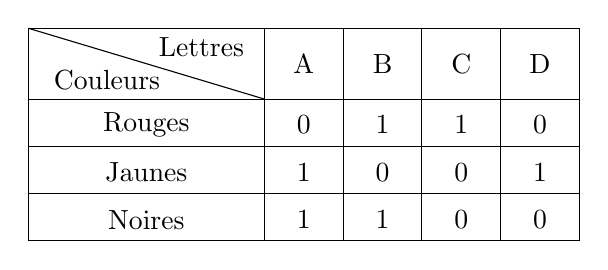
\begin{tikzpicture}[x=1cm,y=.6cm]
            \draw (1,3.5)-- (1,-1);
            \draw (1,-1)-- (8,-1);
            \draw (8,-1)-- (8,3.5);
            \draw (8,3.5)-- (1,3.5);
            \draw (1,2)-- (8,2);
            \draw (8,2)-- (8,0);
            \draw (8,0)-- (1,0);
            \draw (1,0)-- (1,2);
            \draw (1,1)-- (8,1);
            \draw (7,3.5)-- (7,-1);
            \draw (6,-1)-- (6,3.5);
            \draw (5,3.5)-- (5,-1);
            \draw (4,-1)-- (4,3.5);
            \draw (1,3.5)-- (4,2);
            \draw (4.5,2.75) node {A};
            \draw (5.5,2.75) node {B};
            \draw (6.5,2.75) node {C};
            \draw (7.5,2.75) node {D};
            \draw (2.5,1.45) node {Rouges};
            \draw (2.5,0.45) node {Jaunes};
            \draw (2.5,-0.55) node {Noires};
            \draw (3.2,3.1) node {Lettres};
            \draw (2,2.4) node {Couleurs};
            \draw (4.5,1.45) node {0};
            \draw (5.5,1.45) node {1};
            \draw (6.5,1.45) node {1};
            \draw (7.5,1.45) node {0};
            \draw (4.5,0.45) node {1};
            \draw (5.5,0.45) node {0};
            \draw (6.5,0.45) node {0};
            \draw (7.5,0.45) node {1};
            \draw (4.5,-0.55) node {1};
            \draw (5.5,-0.55) node {1};
            \draw (6.5,-0.55) node {0};
            \draw (7.5,-0.55) node {0};
      \end{tikzpicture}%
      }
	  \par\smallskip
      
      Chaque jeton a la m\^eme probabilit\'e d'\^etre tir\'e.
      \begin{description}
            \item[I. ]
                  On tire au hasard et successivement sans remise trois jetons du sac.
                  \begin{enumerate}
                        \item Calculer la probabilit\'e de chacun des \'ev\`enements suivants :
                              \begin{itemize}
                                    \item $E$ : << Obtenir exactement un jeton rouge >>.
                                    \item $F$ : << Obtenir dans l'ordre, les lettres B, A, C >>.
                              \end{itemize}
                        \item Soit $X$ la variable al\'eatoire associ\'ee au rang de la premi\`ere consonne sortie.
                              \begin{enumerate}
                                    \item D\'eterminer l'univers-image de $X$.
                                    \item Etablir la loi de probabilit\'e de $X$ et calculer 
                                          l'esp\'erance math\'ematiques $E(X)$ de $X$.
                              \end{enumerate}
                  \end{enumerate}
            \item[II. ]
                  Une \'epreuve $(E)$ consiste \`a tirer simultan\'ement trois jetons du sac.
                  \begin{enumerate}
                        \item Calculer la probabilit\'e de l'\'ev\`enement : 
                              $G$ : << Obtenir les lettres du mot  B A C >>.
                        \item On répète trois fois de suite et d’une manière indépendante l’épreuve$(E)$.
                              A chaque épreuve, on marque 1 point si l’événement $G$ est réalisé, sinon on marque 0 point.
                              Soit $Y$ la variable aléatoire égale au total des points obtenus à l’issue des trois épreuves.
                              \begin{enumerate}
                                    \item Préciser l'univers-image de $Y$ et déterminer la loi de probabilité de $Y$.
                                    \item Calculer l'espérance mathématique $E(Y)$ de $Y$ puis la variance $V(Y)$ de $Y$. 
                              \end{enumerate}
                  \end{enumerate}
      \end{description}
%%%%%%%%%%%%%%%%%%%%%%%%%%%%%%%%%%%%%%%%%%%%%%%%%%%%%%%%%%%%%%%%%%%%%%%%%%%%%%%%%%%%%%%%%%%%%%%
%%%%%%%%%%%%%%%%%%%                   %%%%%%%%%%%%%%%%%%%                   %%%%%%%%%%%%%%%%%%%
%%%%%%%%%%%%%%%%%%%%%%%%%%%%%%%%%%%%%%%%%%%%%%%%%%%%%%%%%%%%%%%%%%%%%%%%%%%%%%%%%%%%%%%%%%%%%%%
\noindent \underline{\textsc{Probleme}} (10 points) \newline
      On considère la fonction numérique $f$ définie sur  $\mathbb{R}$ par : $f(x) =  (x^2 + 1)\; \expo{-x} + x$.
      On désigne par $\Courbe$ la courbe représentative de $f$ dans un repère orthonormé \Oij{} d'unit\'e $1\cm$.
      \begin{description}
            \item[I. ]
                  Soit $g$ la fonction num\'erique d\'efinie sur $\mathbb{R}$ par : $g(x) = 1 - (x-1)^2\; \expo{-x}$.
                  \begin{description}
                        \item[a)] Calculer $\displaystyle{\lim_{x\rightarrow -\infty} g(x)}$.
                        \item[b)] Montrer que $\displaystyle{\lim_{x\rightarrow +\infty} g(x) = 1}$
                              en admettant que 
                              $\displaystyle{\lim_{x\rightarrow +\infty} \frac{\expo{x}}{x^n} = +\infty},\ n\in\mathbb{N}$.
                        \item[c)] Calculer la d\'eriv\'ee $g'(x)$ de $g$ pour tout $x\in\mathbb{R}$.
                        \item[d)] Dresser le tableau de variation de $g$.
                        \item[e)] Calculer $g(0)$ et en d\'eduire le signe de $g(x)$ pour tout $x \in \mathbb{R}$.
                  \end{description}
            \item[II. ]
                   \begin{enumerate}
                        \item \begin{enumerate}
                                    \item Montrer que $\displaystyle{\lim_{x\rightarrow -\infty} f(x) = +\infty}$
                                          et $\displaystyle{\lim_{x\rightarrow +\infty} f(x) = +\infty}$.
                                    \item Montrer que pour tout $x\in\mathbb{R}$, $f'(x) = g(x)$ et dresser le tableau de 
                                          variation de $f$.
                              \end{enumerate}
                        \item \begin{enumerate}
                                    \item Montrer que le point $A$ d'abscisse $1$ est un point d'inflexion de $\Courbe$.
                                    \item Donner une \'equation de la tangente $(T)$ \`a la courbe $\Courbe$ au point $A$.
                                    \item Montrer que la droite $(\Delta)$ d'\'equation $y=x$ est une asymptote oblique 
                                          \`a $\Courbe$.
                                    \item Etudier la branche infinie de $\Courbe$ en $-\infty$.
                                    \item Tracer $(T)$, $(\Delta)$ et $\Courbe$.
                              \end{enumerate}
                        \item \begin{enumerate}
                                    \item A l'aide d'une double int\'egration par partie,
                                          calculer l'int\'egrale : $I = \int_{0}^{1} x^2 \; \expo{-x} \; \dx$.
                                    \item En d\'eduire l'aire g\'eom\'etrique $A$, en $\cm^2$, du domaine plan limit\'e
                                          par la courbe $\Courbe$, la droite $(\Delta)$ et le droites d'\'equations : 
                                          $x = 0$ et $x = 1$.
                              \end{enumerate}
                        %
                        \begin{center}
                              On donne : $e \simeq 2,7$ ; $\expo{-1} = \frac{1}{e} \simeq 0,4$.
                        \end{center}
                  \end{enumerate}
      \end{description}






